%
%
%Backscattering in microring resonators
%Guillem Ballesteros
%

%%%%%%%%%%%%%%%%%%%%%%% preamble %%%%%%%%%%%%%%%%%%%%%%%%%%%
\documentclass[10pt,letterpaper]{article}
\usepackage{opex3}
\usepackage{amsmath}

\usepackage{color}
\newcommand{\comment}[1]{\textcolor{red}{#1}}
 %\usepackage{ae} %%for Computer Modern fonts

%%%%%%%%%%%%%%%%%%%%%%% begin %%%%%%%%%%%%%%%%%%%%%%%%%%%%%%
\begin{document}

%%%%%%%%%%%%%%%%%% title page information %%%%%%%%%%%%%%%%%%
\title{Characterizing and modeling backscattering in silicon microring resonators}

\author{G. C. Ballesteros$^*$, J. Matres, J. Mart\'i and C. J. Oton}

\address{Nanophotonics Technology Center, \\ Universidad Polit\'ecnica de Valencia, Camino de Vera s/n, 46022, Valencia, Spain}

\email{$^*$guibalga@ntc.upv.es}


%%%%%%%%%%%%%%%%%%% abstract and OCIS codes %%%%%%%%%%%%%%%%
%% [use \begin{abstract*}...\end{abstract*} if exempt from copyright]

\begin{abstract}
We present an experimental technique to characterize backscattering in silicon microring resonators, together with a simple analytical model that reproduces the experimental results. The model can extract all the key parameters of an add-drop-type resonator, which are the loss, both coupling coefficients and backscattering. We show that the backscattering effect strongly affects the resonance shape, and that consecutive resonances of the same ring can have very different backscattering parameters.
\end{abstract}

\ocis{(220.0220) Optical design and fabrication; (230.5750) Resonators; (230.3990) Microstructure devices; (250.5300) Photonic Integrated Circuits.}

%%%%%%%%%%%%%%%%%%%%%%% References %%%%%%%%%%%%%%%%%%%%%%%%%
%\bibliographystyle{osajnl}
%\bibliography{library}
\begin{thebibliography}{10}
\newcommand{\enquote}[1]{``#1''}

\bibitem{Little1998}
B.~E. Little, J.~S. Foresi, G.~Steinmeyer, E.~R. Thoen, S.~T. Chu, H.~A. Haus,
  E.~P. Ippen, L.~C. Kimerling, and W.~Greene, \enquote{{Ultra-Compact Si –
  SiO Microring Resonator},} IEEE Photon. Technol. Lett. \textbf{10}, 549--551 (1998).

\bibitem{DeVos2007}
K.~{De Vos}, I.~Bartolozzi, E.~Schacht, P.~Bienstman, and R.~Baets,
  \enquote{{Silicon-on-Insulator microring resonator for sensitive and
  label-free biosensing},} Opt. Express \textbf{15}, 7610--5 (2007).

\bibitem{So2004}
R.~R.~P. {Vilson R. Almeida, Carlos A. Barrios} and M.~Lipson,
  \enquote{{All-optical control of light on a silicon chip},} Nature
  \textbf{431}, 1081--1084 (2004).

\bibitem{Dumon2004}
P.~Dumon, W.~Bogaerts, V.~Wiaux, J.~Wouters, S.~Beckx, J.~{Van Campenhout},
  D.~Taillaert, B.~Luyssaert, P.~Bienstman, D.~{Van Thourhout}, and R.~Baets,
  \enquote{{Low-Loss SOI Photonic Wires and Ring Resonators Fabricated With
  Deep UV Lithography},} IEEE Photon. Technol. Lett. \textbf{16},
  1328--1330 (2004).

\bibitem{Morichetti2010a}
F.~Morichetti, A.~Canciamilla, M.~Martinelli, A.~Samarelli, R.~M. {De La Rue},
  M.~Sorel, and A.~Melloni, \enquote{{Coherent backscattering in optical
  microring resonators},} Appl. Phys. Lett. \textbf{96}, 081112 (2010).

\bibitem{Little1997a}
B.~E. Little, J.~P. Laine, and S.~T. Chu, \enquote{{Surface-roughness-induced
  contradirectional coupling in ring and disk resonators},} Opt. Lett.
  \textbf{22}, 4--6 (1997).

\bibitem{Kippenberg2002}
T.~J. Kippenberg, S.~M. Spillane, and K.~J. Vahala, \enquote{{Modal coupling in
  traveling-wave resonators},} Opt. Lett. \textbf{27}, 1669--71 (2002).

\bibitem{Zhang2008}
Z.~Zhang, M.~Dainese, L.~Wosinski, and M.~Qiu, \enquote{{Resonance-splitting
  and enhanced notch depth in SOI ring resonators with mutual mode coupling},}
  Opt. Express \textbf{16}, 4621 (2008).

\bibitem{Morichetti2010b}
F.~Morichetti, \enquote{{Roughness Induced Backscattering in Optical Silicon
  Waveguides},} Phys. Rev. Lett. \textbf{104}, 1--4 (2010).

\bibitem{Haus1984}
H.~A. Haus, \emph{{Waves and field in optoelectronics}} (Prentice-Hall, 1984).

\bibitem{J.HeebnerR.Grover2008}
T.~A.~I. {J. Heebner, R. Grover}, \emph{{Optical Microresonators: Theory,
  Fabrication and Applications}} (Springer-Verlag, 2008).

\bibitem{Little1997}
B.~Little, S.~Chu, H.~Haus, J.~Foresi, and J.-P. Laine, \enquote{{Microring
  resonator channel dropping filters},} J. Lightwave Technol.
  \textbf{15}, 998--1005 (1997).

\bibitem{Morichetti2010}
F.~Morichetti, A.~Canciamilla, and A.~Melloni, \enquote{{Statistics of
  backscattering in optical waveguides},} Opt. Lett. \textbf{35}, 1777--9
  (2010).

\bibitem{McKinnon2009}
W.~R. McKinnon, D.~X. Xu, C.~Storey, E.~Post, A.~Densmore, A.~Del\^{a}ge,
  P.~Waldron, J.~H. Schmid, and S.~Janz, \enquote{{Extracting coupling and loss
  coefficients from a ring resonator},} Opt. Express \textbf{17}, 18971--82
  (2009).

\end{thebibliography}
%%%%%%%%%%%%%%%%%%%%%%%%%%%
%%%%%%%%           Introduction           %%%%%%
%%%%%%%%%%%%%%%%%%%%%%%%%%%
\section{Introduction}

Silicon photonics has recently emerged as a viable technology for integrated photonic devices. Microring resonators are elements which are simple to fabricate and are used for devices such as optical filters,~\cite{Little1998} sensors,~\cite{DeVos2007} modulators,~\cite{So2004} etc. The quality factor is usually the parameter that determines the performance of the device; however, in this technology the limiting factor is in most cases not the propagation loss, which can reach values below 2.4~dB/cm~\cite{Dumon2004}, but the backscattering effect due to sidewall roughness~\cite{Morichetti2010a}. Backscattering in a resonator cannot be accounted for as a loss mechanism because in a cavity it grows coherently in each loop. Backscattering is a well known cause of resonance splitting~\cite{Little1997a,Kippenberg2002}; but even before splitting occurs, it can dramatically modify the depth of the resonance; this can sometimes be useful to improve the extinction ratio of the peak~\cite{Zhang2008}. If this effect is not taken into account and one extracts the parameters of the ring from a fit, it can produce a good curve agreement but with wrong results.  In this paper, we propose a characterization technique and a fully analytical fitting procedure that allows a complete characterization of all the parameters of the ring including backscattering, without the need of a coherent backscattering measuring system as in~\cite{Morichetti2010a,Morichetti2010b}.

%%%%%%%%%%%%%%%%%%%%%%%%%%
%%%%%%     Experiment      %%%%%%%%%%%
%%%%%%%%%%%%%%%%%%%%%%%%%%
\section{Experiment}

Silicon waveguides were fabricated through the ePIXfab service at CEA-LETI, France, using silicon-on-insulator  wafers with 220nm Si thickness and 2~$\mu$m buried oxide thickness. Waveguides are fully-etched 220$\times$450nm channels which are covered with a 2~$\mu\textrm{m}$ SiO$_2$ layer, and shallow-etched grating couplers were used for coupling the light vertically from standard single-mode fibers at 10$^\circ$ angle. Waveguides and gratings were both patterned with deep-UV lithography. Transverse-electric (TE) polarization was used in all the experiments. Transmission spectra were collected with a tunable laser with 1~pm resolution and 2~dBm input power in fiber. The rings had a 20~$\mu$m radius and two coupling points, providing a \emph{through} and a  \emph{drop} port. However, in this experiment we also collected the signal from the counter-propagating drop port, which we will call \emph{counter-drop} port (as shown in Fig.~\ref{fig:add_drop_ring}). Measuring this port is crucial to fully characterize the ring, as it directly provides the information about the backscattering inside the cavity. The gap of the through and drop couplers was 275nm and 300nm respectively. 
%%%%%%%%%%%%%%%
\begin{figure}
    \centering
    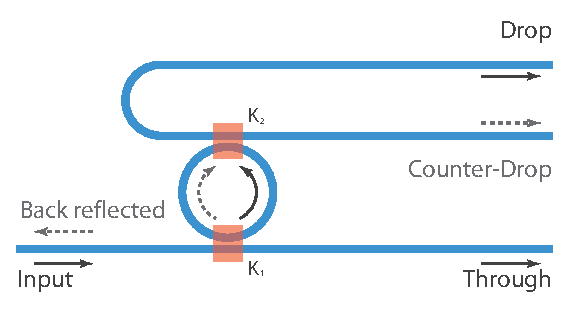
\includegraphics[height=3.3cm,width=7.0cm]{add_drop_ring.eps}
    \caption{(Color online) Schematic view of the layout of add-drop rings with drop (D), counter-drop (C) and through (T) ports. The back reflected port represents the backreflected signal that returns to the \emph{input} port }
    \label{fig:add_drop_ring}
\end{figure}
%%%%%%%%%%%%%%%%%%

Figure~\ref{fig:espectro} shows the measured transmission extracted from all three ports of one microring. It is worth noting that the shape of the resonances is very variable, even though one would expect the loss and the coupling coefficients to be approximately the same in all cases. The reason for this behavior is the backscattering parameter, which is intrinsically noisy, thus producing an apparently random response in their resonances. It is noisy because reflections are produced by sidewall roughness along the ring, so they are randomly distributed along its length, and the overall reflection coefficient results from the interference of all the components, giving rise to sharp spectral variations. In order to extract the parameters of the ring, one must take into account backreflection, otherwise the estimation of the loss and coupling coefficients would depend on which resonance we select, which is unphysical and would produce wrong results. Therefore, a procedure to extract all the parameters including backreflection is needed in order to understand the behavior of our microring resonator. Next section provides an analytical treatment and a recipe to extract all the parameters from any given resonance.

%%%%%%%%%%%%%%%%%%%%%%%%%%%%%%%%%%%%%%%
\begin{figure*}[t]
    \centering
    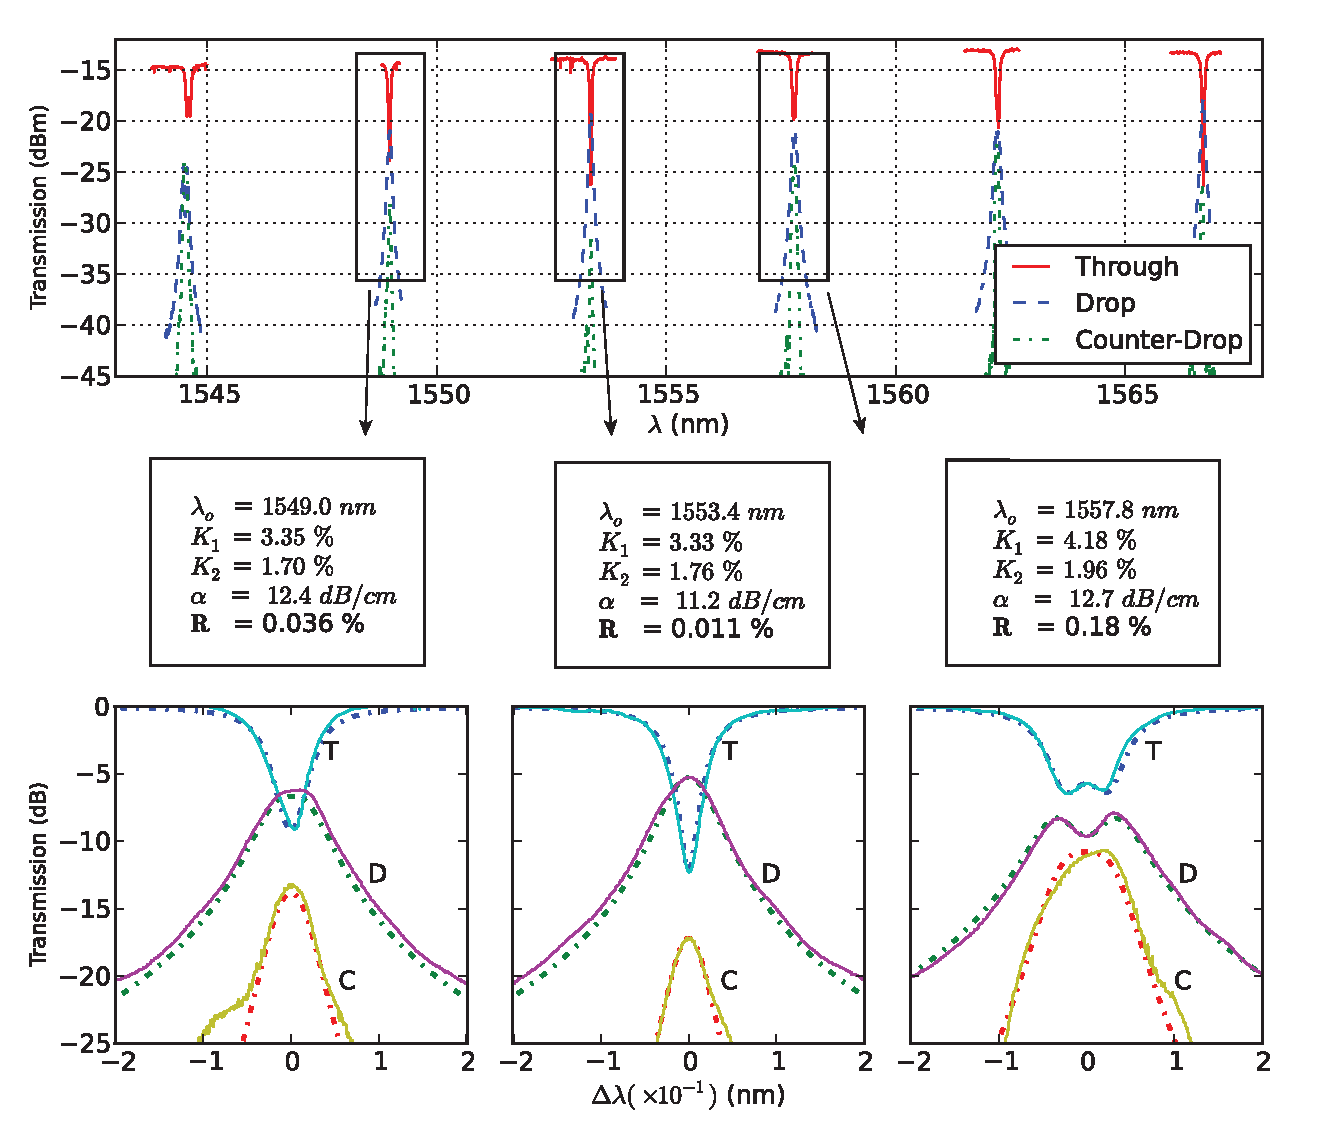
\includegraphics[width=1.0\textwidth, height=11.5cm]{exp_and_fit_data.eps}
    \caption{(Color online)Top panel: Transmission spectrum of each port of the microring: the \emph{through} (red, solid), the \emph{drop} (blue, dashed), and the \emph{counter-drop} (green, dash-dot). Bottom panels: Detail of 3 resonances corresponding to the peaks at 1549, 1553 and 1558~nm, where transmission has been normalized. Solid curves are the experimental data and dashed lines are the analytical curves using the parameters extracted from the fitting procedure and shown on top of each subplot.}

    \label{fig:espectro}

\end{figure*}
%%%%%%%%%%%%%%%%%%%%%%%%%%%%%%%%%%%%%%%


%%%%%%%%%%%%%%%%%%%%%%%%%%%
%%%%%%%%%%         Theory     %%%%%%%%%
%%%%%%%%%%%%%%%%%%%%%%%%%%%
\section{Theory}
\label{sec:theory}

To study this problem we use the time-domain model of two resonators coupled through a coupling constant~\cite{Haus1984}, and we apply it for the ring resonator problem as in Ref.~\cite{Zhang2008}.
Typically time-domain analyses take the photon lifetimes as parameters, but these can be readily related to the more frequently used energy coupling coefficient, $K_j$, and energy propagation loss constant, $\alpha$, of space-domain analyses~\cite{J.HeebnerR.Grover2008} as in~\cite{Little1997}. The reflection coefficient $R$ represents the energy exchanged between the propagating and counter-propagating modes in a single pass through the ring. The coupling constants were assumed to be the same for both the propagating and counter-propagating modes (this is a neccesary condition of a symmetric coupler). The resulting expressions are as follow:

\begin{equation}
    K_j=\frac{\omega_oL}{Q_{e,j} v_g}  \qquad \alpha=\frac{\omega_o}{Q_i v_g} \qquad \sqrt{R}=\frac{\omega_oL}{2Q_rv_g}
\label{eq:space-constants}
\end{equation}

$Q_{e,1}$, $Q_{e,2}$, $Q_{i}$ and $Q_{r}$ are the Q-factors associated to: the coupling with the bottom and top waveguides, the intrinsic losses and the reflection coefficient; $v_g$ is the group velocity of the fundamental mode of the waveguide and can be obtained from the free spectral range (FSR) of the ring. The coupling points are assumed to be lossless, but if there is any excess loss, it can be accounted for as an intrinsic loss in $Q_i$. The model does not require to specify where along the ring the reflection takes place, as the behavior is not affected by the phase of the reflection parameter. However, the fact that reflections occur at randomly localized points has the consequence of introducing a strong dependence of the reflection parameter versus wavelength. The statistical variations of that parameter have been studied in Ref.~\cite{Morichetti2010}. Q-factors can be related to the $\tau$ constants of the different processes through $Q_j=\omega_o \tau_j/2$. Defining the total quality factor of the ring as:

\begin{equation}
	    \frac{1}{Q}=\frac{1}{Q_{e,1}}+\frac{1}{Q_{e,2}}+\frac{1}{Q_i}
\label{eq:Q_def}
\end{equation}

and following the guidelines in~\cite{Haus1984,Little1997,Zhang2008}, one can obtain the analytical expressions for the output in each port as a function of all the Q-factors previously defined:
\begin{subequations}
\label{eq:ports}
\begin{align}
	T=& \left\lVert1-\frac{        \frac{2}{Q_{e,1}}(2j(\omega '-1)+\frac{1}{Q})   }  {   (2j(\omega '-1)+\frac{1}{Q})^2+\frac{1}{Q_r^2}  }\right\rVert^2 \label{eq:T} \\
	D =& \left\lVert\frac{          \frac{2}{\sqrt{Q_{e,1}Q_{e,2}}}(2j(\omega '-1)+\frac{1}{Q})   }  {   (2j(\omega'-1)+\frac{1}{Q})^2+\frac{1}{Q_r^2}    }\right\rVert^2 \label{eq:D} \\
	C=& \left\lVert\frac{          \frac{2}{Q_r\sqrt{Q_{e,1}Q_{e,2}}}   }  {   (2j(\omega'-1)+\frac{1}{Q})^2+\frac{1}{Q_r^2}    }\right\rVert^2 \label{eq:CD}
\end{align}
\end{subequations}

where $\omega'=\omega/\omega_0$ is the normalized angular frequency of the resonance under study, and $T$, $D$ and $C$ are respectively the energy transmission coefficients of the \emph{through}, \emph{drop} and \emph{counter-drop} ports as defined in Fig.~\ref{fig:add_drop_ring}. Also, Eq.~(\ref{eq:CD}) would yield the \emph{back reflected} energy by multiplying it by $K_1/K_2$. This means that the \emph{counter-drop} port can be used as an indirect measurement of the latter; which can be useful because measuring it directly is not straightfoward as other sources of backscattering (e.g. reflection in the input grating) can hinder the measurement, thus coherent methods as in \cite{Morichetti2010a} are needed.


One way to extract the ring parameters from the experiment would be to find the parameters that produce the best fit to the experimental curves; however fitting three curves simultaneously is not straightforward. For this reason, we have calculated all the Q-factors of the ring as a function of specific values which are easily extracted from the experimental curves, which are the central values of the three ports ($T_0$, $D_0$ and $C_0$, all measured at $\omega_0$), and the parameter $\Delta\omega'$, defined as the normalized frequency width between the points where $C = C_0/2$. When the peak has not yet split, this corresponds to the full-width at half maximum (FWHM) of the \emph{counter-drop} resonance peak. However, if the peak is split in two, the maximum is not located at $C_0$, thus $\Delta\omega'$ would not be the FWHM anymore, although the expressions are still valid using its mathematical definition. After some algebraic manipulation, the equations that allow extracting all the parameters from the experimental curves are the following:

\begin{subequations}
\label{Qfactors}
\begin{align}
    Q=&\frac{1}{\Delta\omega'}\left(\frac{C_o}{D_o}-1 + \sqrt{2}\sqrt{\left(\frac{C_o}{D_o}\right)^2+1}\right)^{1/2} \label{eq:Q} \\
\displaybreak[0]
    Q_r=&\frac{1}{Q}\sqrt{\frac{D_o}{C_o}} \label{eq:Qu}\\
\displaybreak[0]
    Q_{e,1}=&\frac{2}{Q(Q^{-2}+Q_r^{-2})(1\pm\sqrt{T_o})}  \label{eq:Qe1}\\
    Q_{e,2}=&\frac{2(1\pm\sqrt{T_o})}{QD_o(Q^{-2}+Q_r^{-2})}  \label{eq:Qe2}
\end{align}
\end{subequations}


Once all the Q-factors are calculated, one can relate them to the loss, coupling coefficients and backreflection by using Eqs.~(\ref{eq:space-constants}) and (\ref{eq:Q_def}). The sign ambiguity in Eqs.~(\ref{eq:Qe1}) and (\ref{eq:Qe2}) is a byproduct of the existence of two degenerate operation regimes in the ring with different parameters but the same resonance shape. This ambiguity is well known in cases without any backreflection effect, and it is due to the fact  that in some cases one cannot distiguish between the intrinsic and the extrinsic loss. Some possible solutions to overcome this problem are proposed in \cite{McKinnon2009}, and consist in looking at the dependence on wavelength or measuring rings with different geometrical parameters. In our case, the ambiguity only occurs for the peak with lowest reflection coefficient, as in the other two cases it would give rise to a negative loss coefficient, which is unphysical, because it requires gain from the medium. As the sign has to be the same in all the peaks of the same ring, this provides an additional way to decide the correct sign in the expressions by analyzing more than one peak and looking for non-physical solutions.



Looking at Eqs.~(\ref{eq:ports}), one can identify 3 main regimes of operations in which the ring can work. They are distinguished by how strong the backreflection is in relation to the total Q-factor, that is, how large $Q_r$ is in comparison with $Q$. In the case where $Q_r \gg Q$, the coupling can be considered to be negligible and the parameters can be extracted with already existing methods like in~\cite{McKinnon2009}, or by making $1/Q_r=0$ in Eq.~(\ref{eq:T}) and solving for $Q_{e,1}$ and $Q$ as a function of the extinction ratio and the full-width at half depth (FWHD). In this situation all resonances tend to have approximately the same shape and they do not split up. When the intention is to achieve high quality factors, then $Q$ can start to approach to $Q_r$ and the expressions described in this paper should be used. Nevertheless, it may not be obvious from a measurement of a single resonance of the through port that the latter is the actual mode of operation since resonances do not always split; under these circumstances one should look at different peaks and see if they vary in an apparently random fashion, and where possible, measure the \emph{counter-drop} port response. In the case where the coupling is so strong that $Q_r \ll Q$, which may happen if the rings are intentionally designed for this purpose, then simplified expressions can be found as well, which are more practial than Eqs.~(\ref{Qfactors}).  If this is the case then splitting is very evident showing two clearly defined peaks around each resonance frequency. Table~\ref{tab:summary} summarizes the three operation regimes and the expressions to use in each case.

%%%%%%%%%%%%%%%%%%%%%%
%%%%%%        Results        %%%%%%%
%%%%%%%%%%%%%%%%%%%%%%

\section{Results}

From the experimental data shown in Fig.~\ref{fig:espectro}, we have chosen three consecutive resonances which show quite different behavior in terms of extinction ratio and degree of splitting. The results obtained from the method described in section~\ref{sec:theory} for each resonance are also shown in Fig.~\ref{fig:espectro}, and the corresponding theoretical curves are shown in the insets, where a good agreement is observed. It is worth noting that the coupling constants and the loss show small variations among resonances, being $R$ the one showing much higher variability (reaching one order of magnitude). This is expected from the nature of backscattering, and is a demonstration of the validity of our model. The asymmetry of the shape of peaks 1 and 3, which is not reproduced in the theory, can be explained by sudden variations in the reflection coefficient along the width of the resonance, which was not considered in the model.

The maximum reflection coefficient measured is 0.18\%, which corresponds to $Q_r \sim 25~000$. This means that for this waveguide section and quasi-TE polarization, resonances with Q-factors higher than $10^4$ will be affected by backscattering. If one requires pure resonances with higher Q-factors, waveguides with weaker backscattering are needed, which can be achieved by using quasi-TM polarization or by widening the channel.\cite{Morichetti2010b}

%%%%%%%%%%%%%%%%%%%%
%%%%%    Conclusion     %%%%%%%
%%%%%%%%%%%%%%%%%%%%

%%%%%%%%%%%%%%%%%%
%%Tabla resumen

\begin{table}[ht]
	\renewcommand{\arraystretch}{1.3}
	\caption{Summary of expressions for calculating Q-factors of ring-resonators working under different backscattering regimes}
	\centering
	\begin{tabular}{ccccc}
	\hline
	Weak coupling && Intermediate coupling && Strong coupling\\
	$(Q_r \gg Q)$ && $(Q_r \sim Q)$ && $(Q_r \ll Q)$\\
	\cline{1-1} \cline{3-3} \cline{5-5}
	$Q=1/\Delta\omega'_{\mbox{\scriptsize{FWHM}},D}\footnotemark[1]$&&$Q$ (Eq.~(\ref{eq:Q}))&&$Q=1/\Delta\omega'_{\mbox{\scriptsize{FWHM}}}$\\
	$Q_r$ (Eq.~(\ref{eq:Qu}))&&$Q_r$ (Eq.~(\ref{eq:Qu}))&&$Q_r=1/\Delta\mbox{splitting   }\footnotemark[2]$\\
	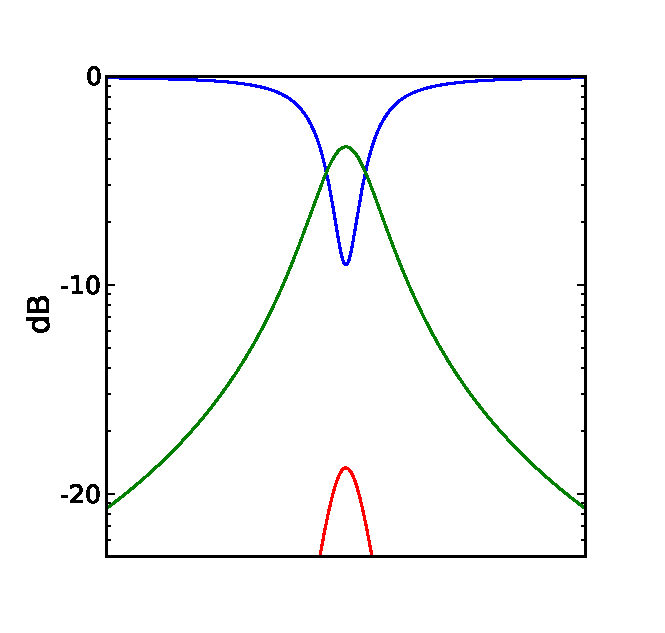
\includegraphics[scale=0.3]{graphic0.eps}&&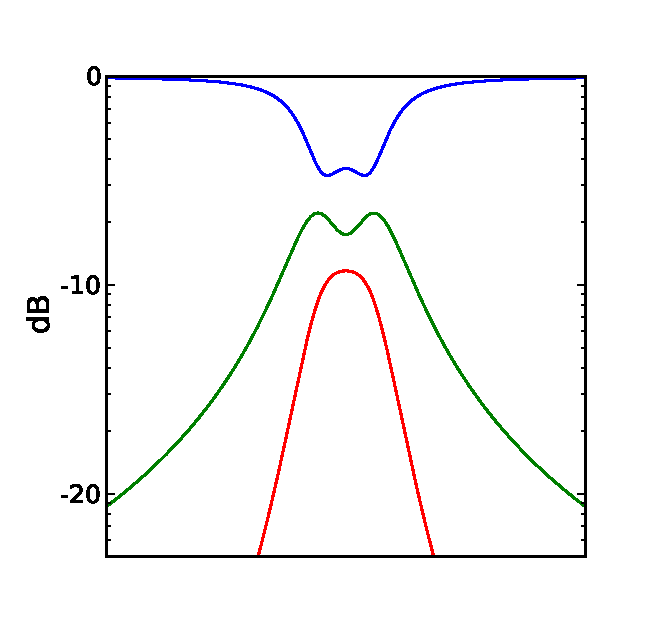
\includegraphics[scale=0.3]{graphic1.eps}&&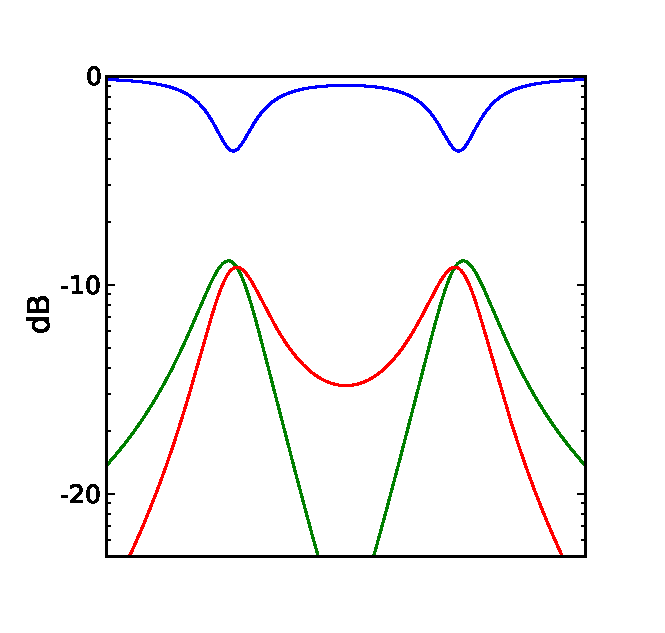
\includegraphics[scale=0.3]{graphic2.eps}\\
	\hline
	\multicolumn{4}{l}{\footnotemark[1]{\footnotesize{Full-width at half maximum of the drop port}}}  \\
	\multicolumn{2}{l}{\footnotemark[2]{\footnotesize{Peak to peak distance}}}
	\end{tabular}
	\label{tab:summary}

\end{table}%
%%%%%%%%%%%%%%%%%%%%%%%%


\section{Conclusion}
We have described an analytical model and a fitting procedure that allows extraction of all the key parameters of a silicon microring resonator with two coupling points. These parameters are the two coupling constants, propagation loss and the backscattering coefficient. With this method, we demonstrate that variations of the backscattering  parameter are the cause of the strong variations in the shape of different resonances of the same microring. All these parameters can be extracted from simple measurements using a standard transmission characterization setup, and the experimental results from a ring resonator are succesfully fitted to the analytical model.


\section*{Acknowledgments}


The authors acknowledge financial support from the Spanish Ministry of Science and Innovation through contract SINADEC (TEC2008-06333). Joaquin Matres is supported by the Formaci\'on de Personal Investigador grant program of the Universidad Polit\'ecnica de Valencia.

\end{document} 
